\section{Additional Qualitative and Benchmark Results}
\label{app:additional_results}



\subsection{Qualitative Analysis for Zero-Shot Cross-Embodiment Experiments}
We present additional qualitative comparisons of all baseline policies under zero-shot embodiment transfer, complementing the results in Section~\ref{subsec:zero_shot}. 
OpenVLA~\cite{kim2024openvlaopensourcevisionlanguageactionmodel}, MolmoAct~\cite{lee2025molmoactactionreasoningmodels}, and $\pi_{0.5}$-Base \cite{intelligence2025pi05visionlanguageactionmodelopenworld} consistently fail to produce meaningful motions across all robot platforms. 
X-VLA~\cite{zheng2025xvlasoftpromptedtransformerscalable} generates smooth trajectories and occasionally approaches target objects on the DROID and Custom Franka setups; however, it never achieves accurate gripper–object alignment required for successful manipulation.

The $\pi_{0}$-replicated baseline exhibits highly imprecise end-effector control. For instance, in the \emph{Tissue} task on the YAM robot, it frequently overshoots the target and grasps the tissue box rather than the tissue itself. In contrast, $\pi_{0.5}$-replicated generally produces smoother and more directionally reasonable motions, but still lacks the spatial precision required for reliable grasping and successful task completion. Across the Custom Franka and Kinova robots, both baselines similarly exhibit imprecise motions, suggesting limited ability to infer accurate control actions under embodiment shift. These failure modes are consistent across all evaluated embodiments. An example rollout is shown in Fig.~\ref{fig:baseline-rollout-visualization}.

\begin{figure*}[h]
    \centering
    \includegraphics[width=\linewidth]{figures/appendix/fig12_baseline_rollout.pdf}
   \caption{\textbf{Example baseline rollout failures on the Sort task (YAM robot).} 
    Both $\pi_{0}$-replicated and $\pi_{0.5}$-replicated exhibit imprecise end-effector control, moving directly toward the basket without first grasping any objects. 
    In contrast, LAP-3B successfully completes the task under similar initial conditions. 
    Open-sourced VLA baselines are omitted as they do not generate meaningful or safe control actions in this setting.}
    \label{fig:baseline-rollout-visualization}
\end{figure*}
\vspace{-5pt}

% \begin{figure}[h]
%     \centering
%     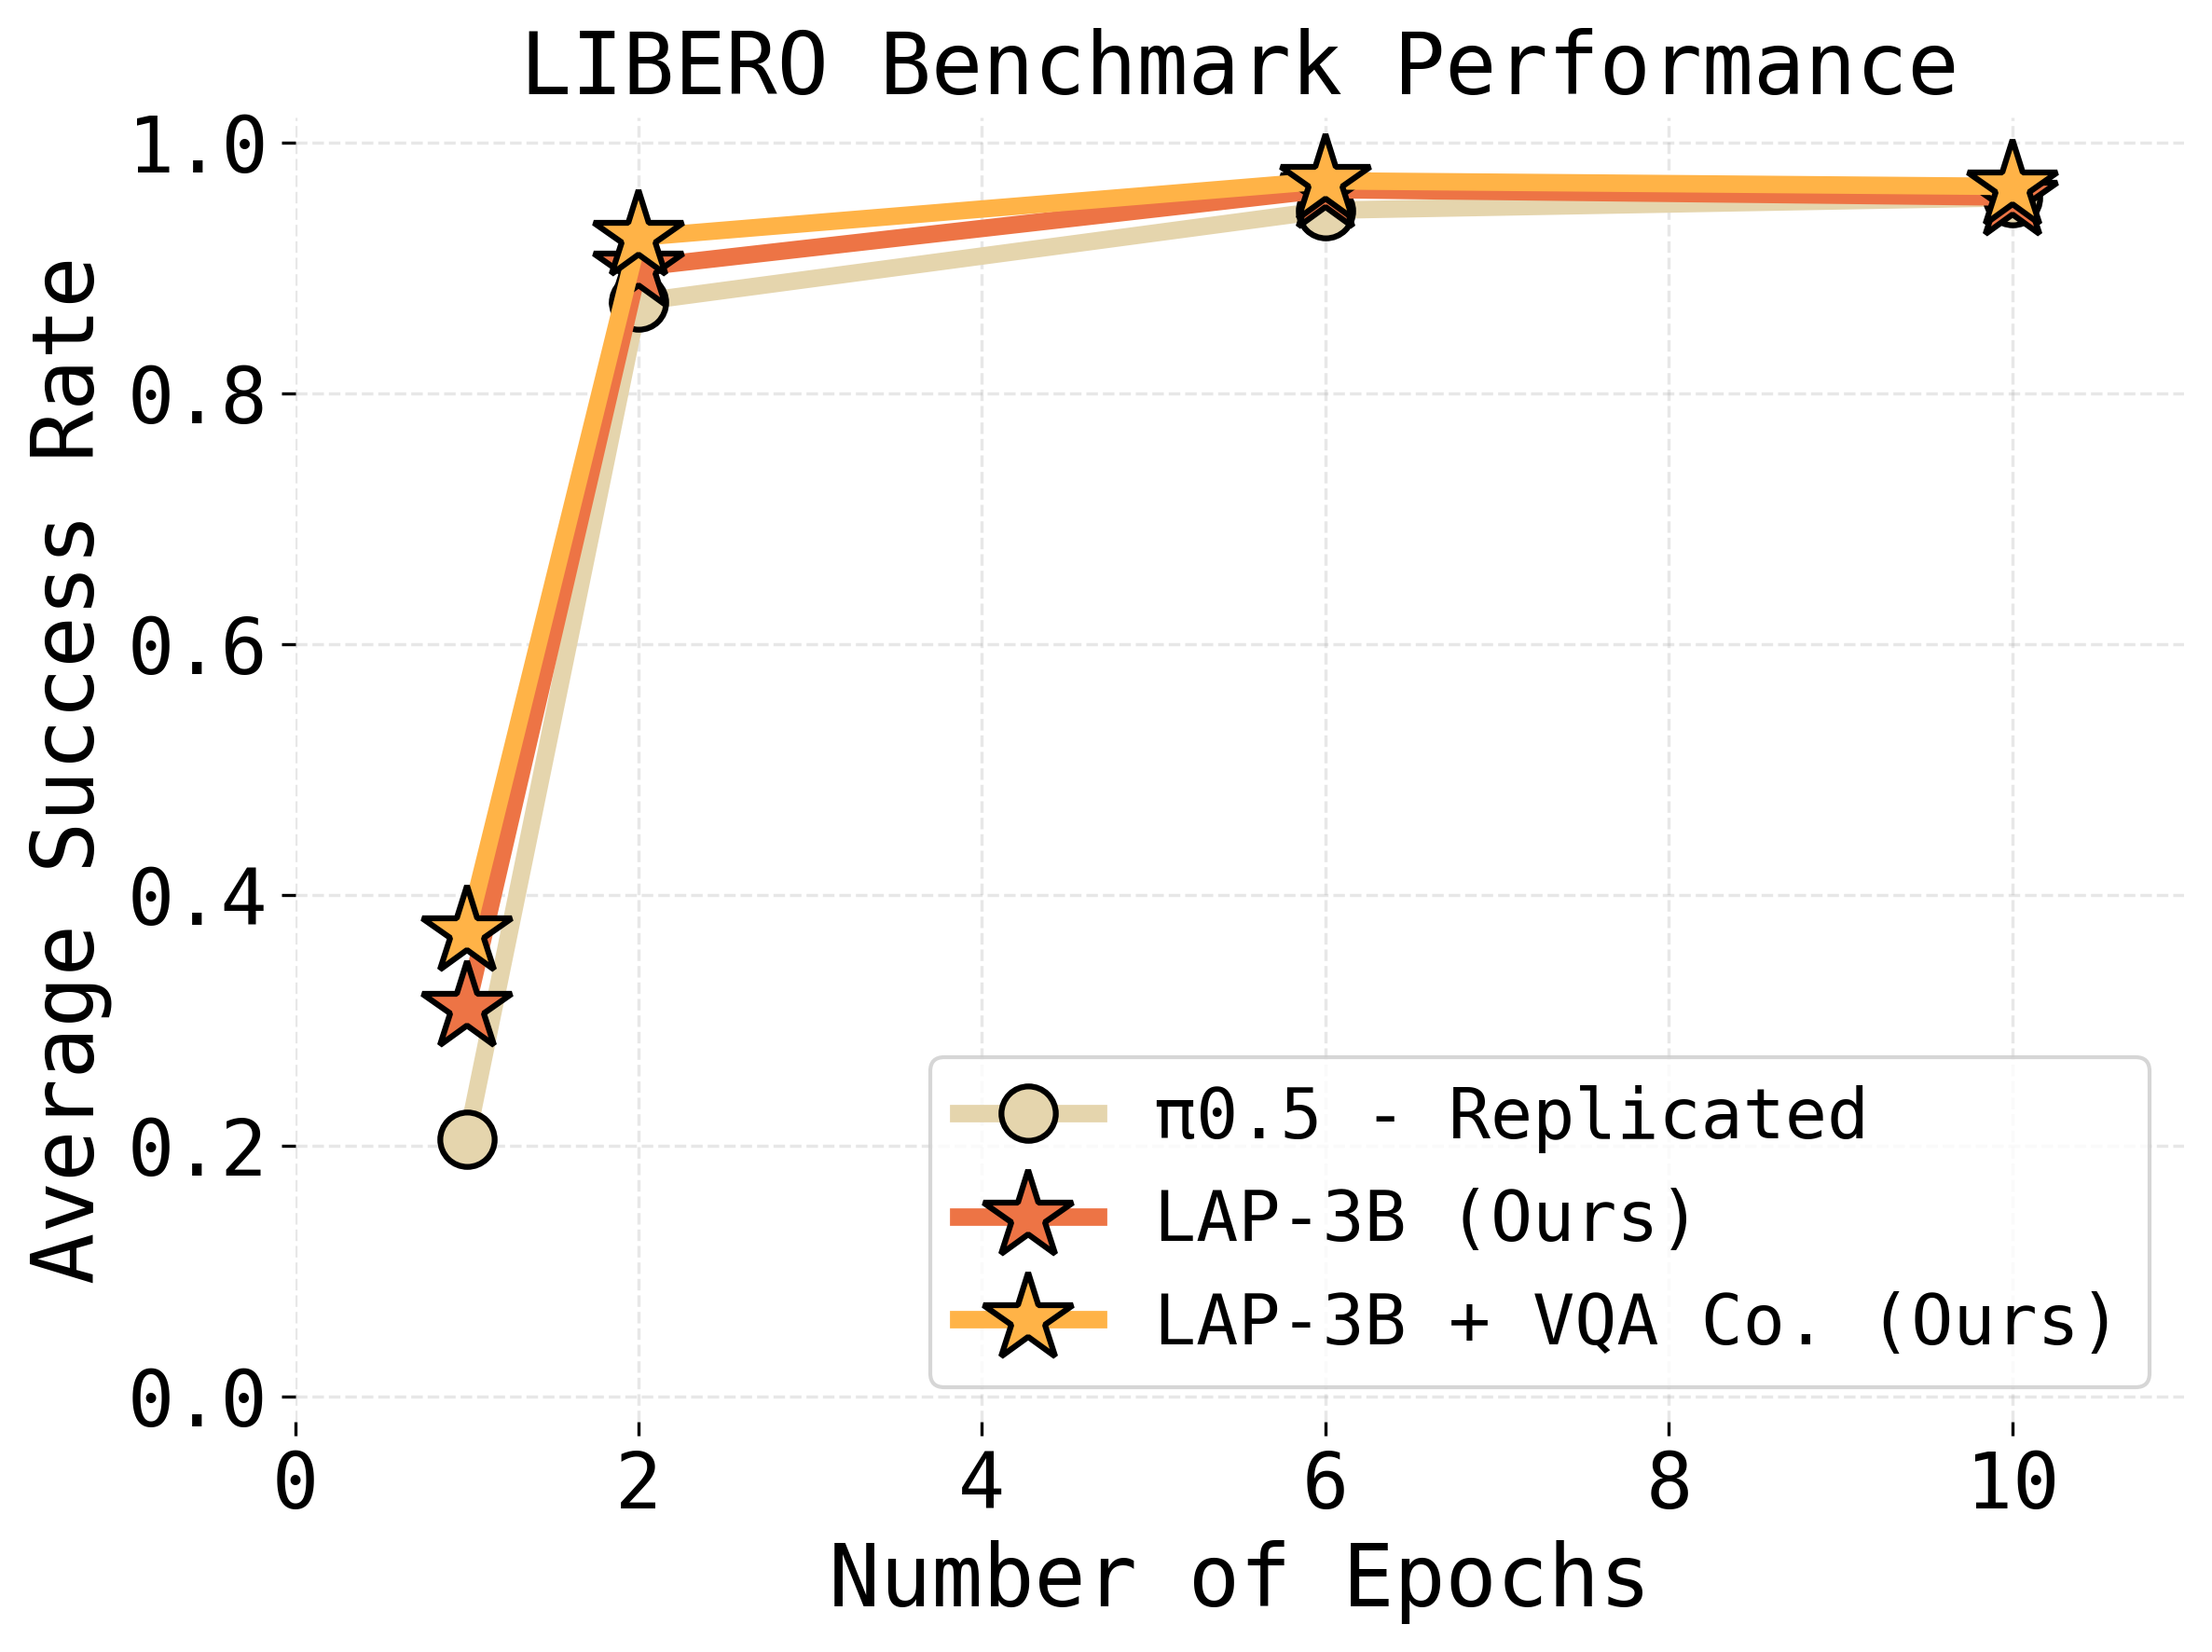
\includegraphics[width=\linewidth]{figures/appendix/fig14_libero_cotrain.png}
%     \caption{\textbf{Compute efficiency on the LIBERO benchmark.} Co-training with VQA data significantly accelerates convergence, enabling \textsc{LAP-3B}+VQA Co-training to achieve high success rates in fewer gradient steps than \textsc{LAP-3B}. For clarity, we report only the strongest replicated baseline ($\pi_{0.5}$-replicated).}
%     \vspace{-8pt}
%     \label{fig:libero-cotraining}
% \end{figure}


\begin{figure*}[b]
    \centering
    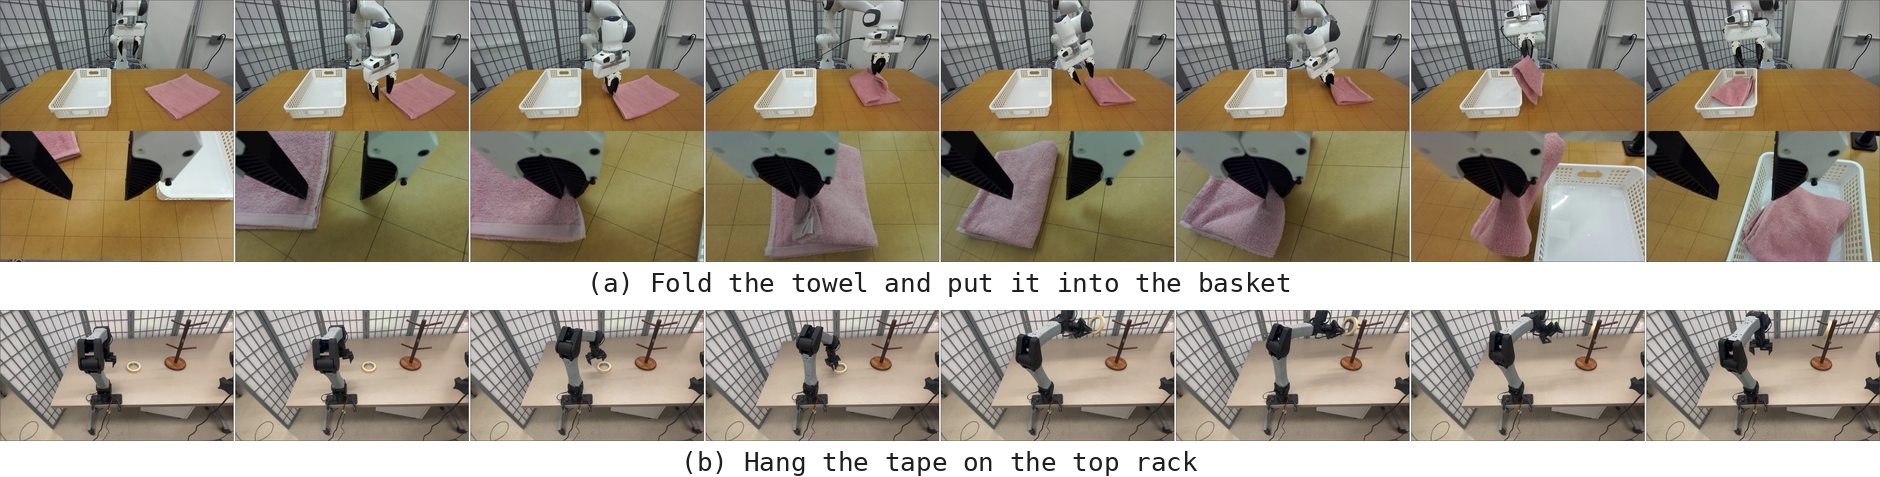
\includegraphics[width=\linewidth]{figures/appendix/fig11_finetune_rollout.png}
    \caption{\textbf{Fine-tuning evaluation rollout visualizations.} Example observations from the camera views used for policy evaluation across different robot embodiments and tasks, shown from left to right.}
    \label{fig:finetuning-rollout-visualization}
\end{figure*}
\vspace{2pt}


\begin{table}[!h]
\centering
\footnotesize
\setlength{\tabcolsep}{4pt}
\caption{LIBERO benchmark results comparing LAP-3B with other state-of-the-art VLAs. Each data point corresponds to an average over 500 trials. Best per column is bolded. Rank is based on Avg. performance (higher is better).}
\begin{tabular}{l c c c c c c}
\toprule
Method & Spatial & Object & Goal & LIBERO-10 & Avg. & Rank \\
\midrule

TraceVLA \cite{zheng2025tracevlavisualtraceprompting} 
& 84.6 & 85.2 & 75.1 & 54.1 & 74.8 & 13 \\

X-VLA \cite{zheng2025xvlasoftpromptedtransformerscalable} 
& 98.2 & 98.6 & 97.8 & \textbf{97.6} & \textbf{98.1} & 1 \\

Octo \cite{octomodelteam2024octoopensourcegeneralistrobot} 
& 78.9 & 85.7 & 84.6 & 51.1 & 75.1 & 12 \\

UniAct \cite{zheng2025universalactionsenhancedembodied} 
& 77.0 & 87.0 & 77.0 & 70.0 & 77.8 & 11 \\

GR00T-N1 \cite{nvidia2025gr00tn1openfoundation} 
& 94.4 & 97.6 & 93.0 & 90.6 & 93.9 & 8 \\

OpenVLA \cite{kim2024openvlaopensourcevisionlanguageactionmodel} 
& 84.7 & 88.4 & 79.2 & 53.7 & 76.5 & 10 \\

OpenVLA-OFT \cite{kim2025finetuningvisionlanguageactionmodelsoptimizing} 
& 97.6 & 98.4 & 97.9 & 94.5 & 97.1 & 3 \\

UniVLA \cite{bu2025univlalearningacttaskcentric} 
& 95.4 & 98.8 & 93.6 & 94.0 & 95.4 & 6 \\

$\pi_0$ \cite{black2024pi0visionlanguageactionflowmodel} 
& 96.8 & 98.8 & 95.8 & 85.2 & 94.2 & 7 \\

$\pi_{0.5}$ \cite{intelligence2025pi05visionlanguageactionmodelopenworld} 
& 98.8 & 98.2 & 98.0 & 92.4 & 96.9 & 4 \\

VLA-0 \cite{goyal2025vla0buildingstateoftheartvlas} 
& 97.0 & 97.8 & 96.2 & 87.6 & 94.7 & 9 \\

% \midrule
% \multicolumn{7}{l}{\underline{\textit{Replicated / Oracle Baselines}}} \\

% $\pi_0$-replicated 
% & 96.8 & 98.4 & 95.6 & 87.2 & 94.5 & -- \\

% $\pi_{0.5}$-replicated 
% & 96.0 & \textbf{99.6} & 97.8 & 90.8 & 96.1 & -- \\

% \textcolor{gray}{$\pi_{0.5}$-Oracle} 
% & \textcolor{gray}{\textbf{99.8}} 
% & \textcolor{gray}{98.6} 
% & \textcolor{gray}{\textbf{99.2}} 
% & \textcolor{gray}{\textbf{96.0}} 
% & \textcolor{gray}{\textbf{98.4}} 
% & -- \\

\midrule
\textbf{\textsc{LAP-3B}} 
& 98.2 & \textbf{99.0} & \textbf{98.8} & 91.2 & 96.8 & 5 \\

\textbf{\textsc{LAP-3B}+ VQA Co.} 
& \textbf{99.0} & \textbf{99.0} & 97.2 & 93.4 & 97.2 & 2 \\

\bottomrule
\end{tabular}
\label{tab:libero_full}
\end{table}




\subsection{Full Results for the LIBERO Benchmark}
\begin{wrapfigure}{r}{0.4\textwidth}
    \centering
    \vspace{-20pt}
    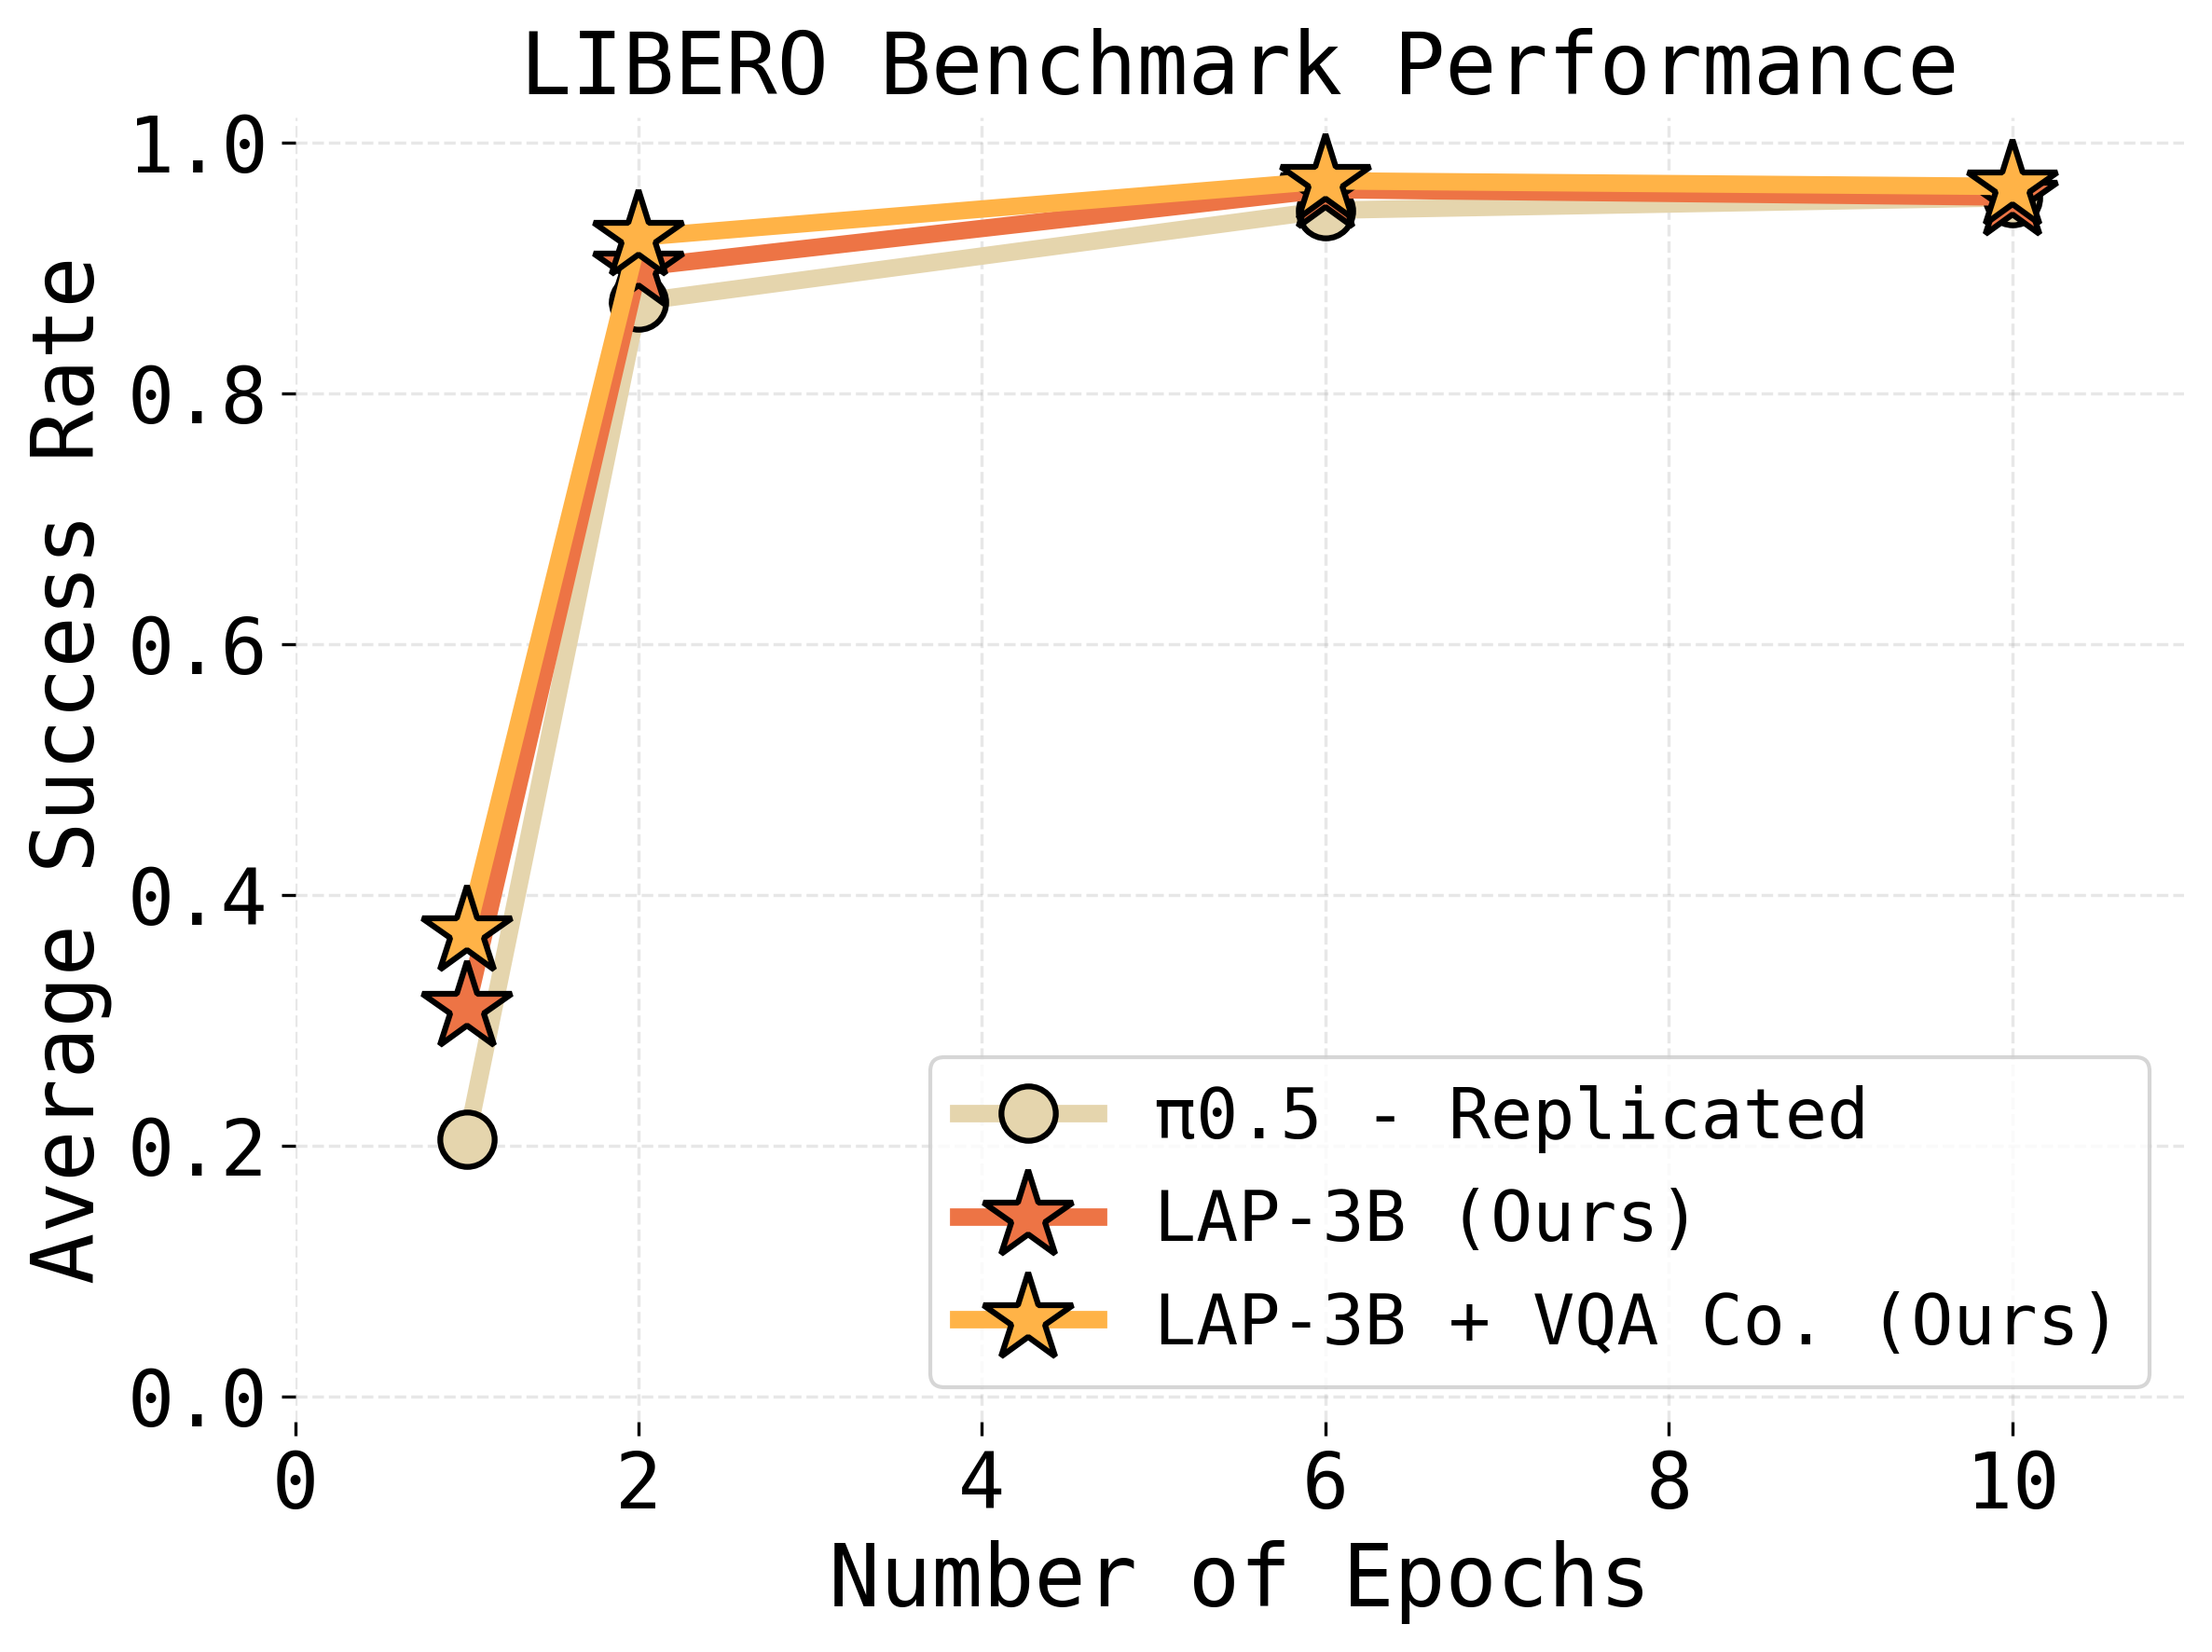
\includegraphics[width=0.4\textwidth]{figures/appendix/fig14_libero_cotrain.png}
    \captionsetup{skip=2pt}
    \caption{\textbf{Compute efficiency on LIBERO.} Co-training with VQA data significantly accelerates convergence, enabling \textsc{LAP-3B}+VQA Co-training to reach high success rates in fewer gradient steps. For clarity, we report only the strongest baseline ($\pi_{0.5}$-replicated).}
    \vspace{-1cm}
    \label{fig:libero-cotraining}
\end{wrapfigure}
Table~\ref{tab:libero_full} reports the complete LIBERO benchmark results, including additional open-source VLA baselines not shown in the main paper, and further confirms the consistent performance gains of \textsc{LAP-3B} across task families and all three task suites. \textsc{LAP-3B}+VQA Co. denotes the policy co-trained with VQA data as described in Section~\ref{sec:experiments}. Its improved performance over \textsc{LAP-3B} alone further underscores the effectiveness of VQA co-training. Moreover, the co-trained checkpoint substantially improves fine-tuning efficiency on LIBERO, achieving stronger performance with the same gradient steps, as shown in Fig.~\ref{fig:libero-cotraining}.


\subsection{Real-Robot Rollouts}
We further provide extended qualitative rollout visualizations across all embodiments and tasks for fine-tuning evaluation in Fig.\ref{fig:finetuning-rollout-visualization} and zero-shot evaluation in Fig.~\ref{fig:zeroshot-rollout-visualization}. 
Each panel corresponds to the camera views used during policy execution. 


